\begin{frame}
	\frametitle{Detección de Keypoints}
	
	\note{https://youtu.be/ebMyBbkkHWk}
	
	\note{https://3d.bk.tudelft.nl/courses/geo1016/slides/Lecture_03_Calibration.pdf}
	
	\footnotesize
	Propiedades deseables para SLAM / SfM:
	\begin{itemize}
		\item Alta repetitibilidad
		\item Alta precisión
		\item Robustez
		\item Invarianza (luminosidad, puntos de vista, etc)
		\item Computacionalmente eficientes
		\item Algunos detectores: HARRIS, SIFT, SURF, Shi-Tomasi, FAST, ORB, BRISK
	\end{itemize}

	
	\begin{figure}
		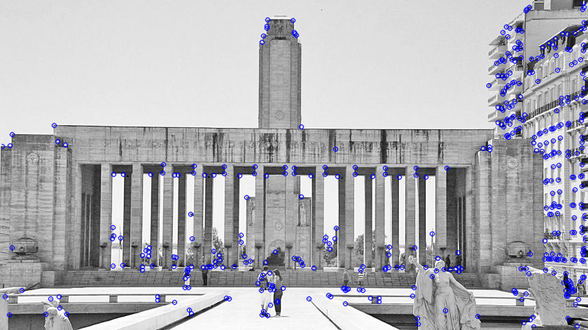
\includegraphics[width=0.5\textwidth]{./images/keypoints_fast}
		\caption{Keypoints FAST}
	\end{figure}

\end{frame}


\begin{frame}
	\frametitle{Matcheo de keypoints}
	\footnotesize
	Propiedades deseables del matcheo de keypoints para SLAM / SfM:
	\begin{itemize}
		\item Alto recall
		\item precisión
		\item Robustez
		\item Computacionalmente eficientes
		\item Posibles enfoques: patches o descriptores
	\end{itemize}
	
	\begin{figure}
		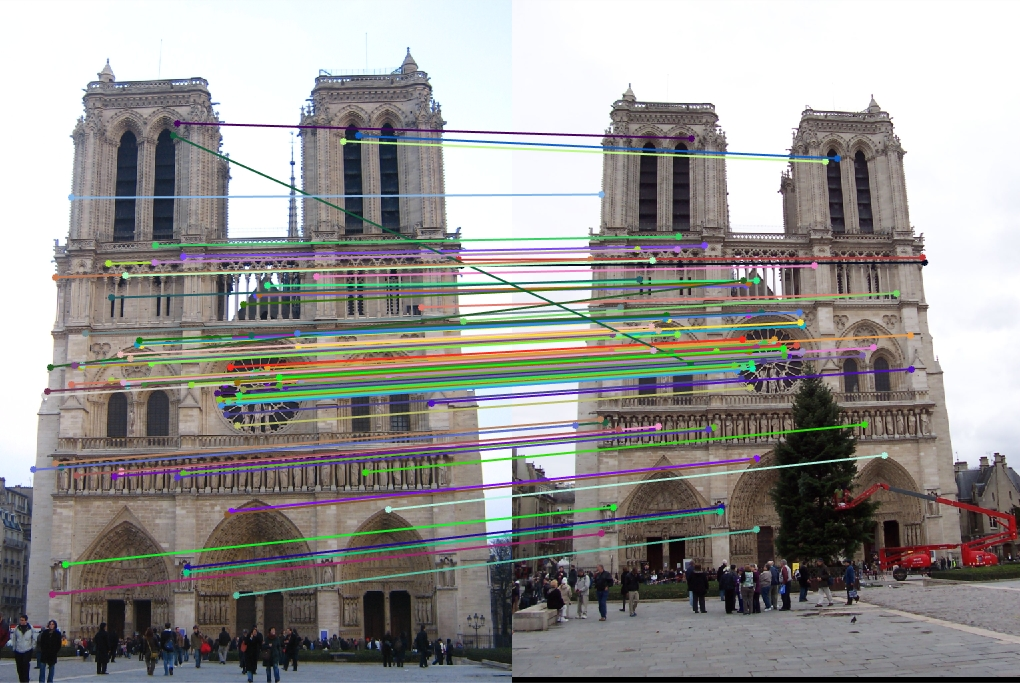
\includegraphics[width=0.4\textwidth]{./images/matching_notredam.jpg}
		\caption{Keypoints Harris + Descriptor SIFT}
	\end{figure}
	\note{Imagen extraida de https://www.cc.gatech.edu/classes/AY2016/cs4476_fall/results/proj2/html/cpolack6/index.html}
\end{frame}

\begin{frame}
	\frametitle{Precision - Recall}
	\footnotesize
	
	\note{https://upload.wikimedia.org/wikipedia/commons/2/26/Precisionrecall.svg}
	
	\begin{figure}
		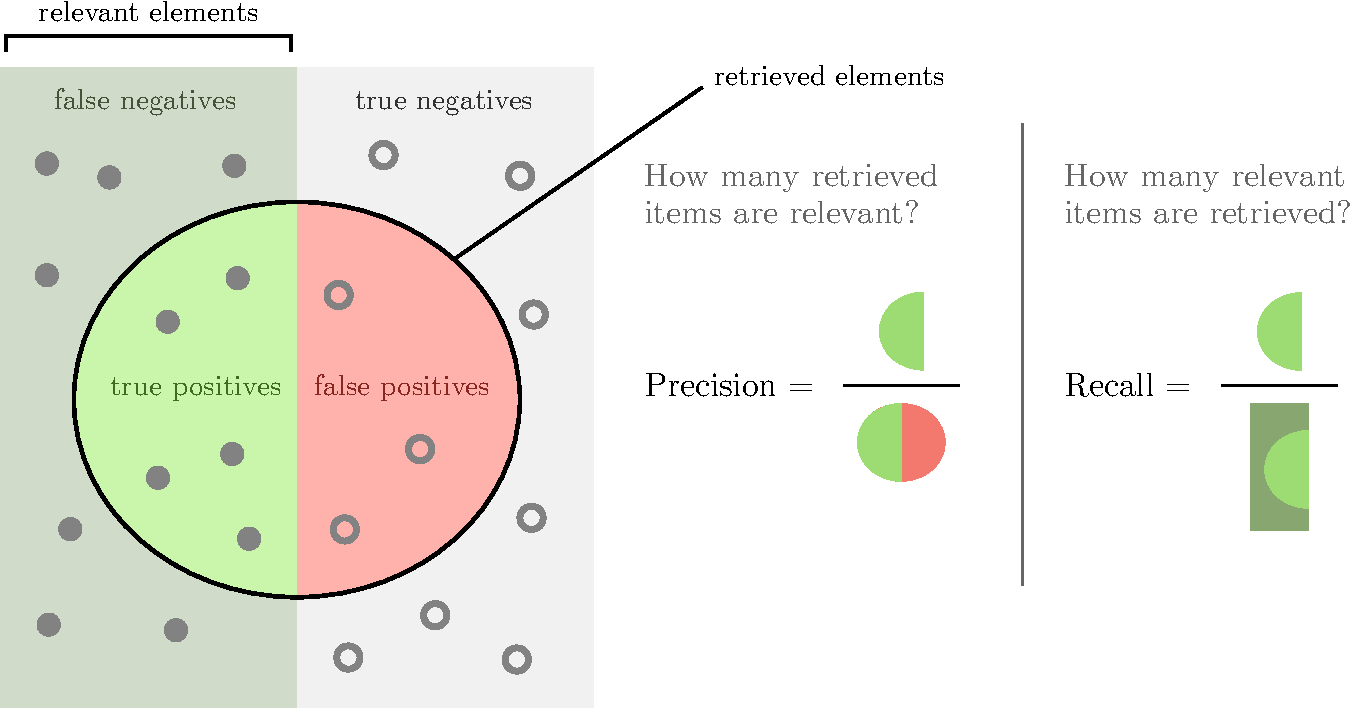
\includegraphics[width=0.25\textwidth]{./images/precision_recall.pdf}
	\end{figure}
\end{frame}

\begin{frame}
	\frametitle{Desciptores de features Locales}
	\footnotesize
	
	Propiedades deseables para SLAM / SfM: distinguibles, robustos, invariantes
	\begin{itemize}
		\item Extraer firmas sobre regiones de la imagen ejemplos:
		\begin{itemize}
			\item Histogramas sobre gradientes de la imagen (SIFT)
			\item Histogramas sobre respuestas Haar-wavelet (SURF)
			\item Patrones binarios (BRIEF, BRISK, FREAK, ORB)
			\item Descriptores basados en aprendizaje
		\end{itemize}
		\item Invariante rotación: Alineado con la orientación dominante de la región local
		\item Invariante a escala: Adaptar la región descripta a la escala de keypoint
	\end{itemize}

	\TODO{agregar imagenes SIFT BRIEF}
	
\end{frame}

\begin{frame}
	\frametitle{Local Features invariantes}
	\footnotesize
	
	\begin{itemize}
		\item Invarianza geométrica: traslación, rotación, escala.
		\item Invarianza fotométrica: brillo, exposición, etc.
	\end{itemize}
	 

\end{frame}

\begin{frame}
	\frametitle{Ventajas de features locales}
	\footnotesize

	\begin{itemize}
	\item Locales: los features al ser locales son robustos a oclusiones
	\item Distintivos: pueden diferenciar un gran conjunto de objetos
	\item Cuantiosos: puede haber cientos o miles en una misma imagen
	\item Eficientes: al discretizar la imagen, se puede obtener tiempo real.
\end{itemize}
	
\end{frame}

\begin{frame}
	\frametitle{Harris}
	\footnotesize
	
	\TODO{Agregar slides de SIFT, HARRIS, FAST y ORB https://youtu.be/ebMyBbkkHWk}
	
\end{frame}

\begin{frame}
	\frametitle{Características Visuales: Detector FAST}
	
	\begin{figure}
		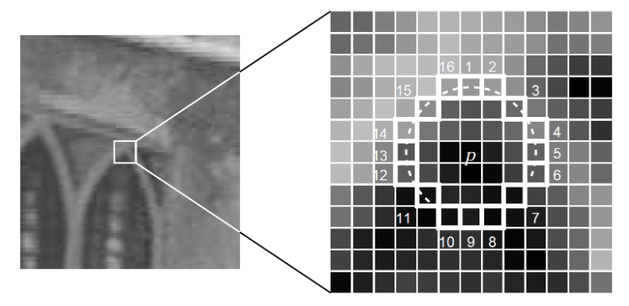
\includegraphics[width=0.8\textwidth]{./images/camera/fast}
	\end{figure}
	
	El valor de intensidad del pixel $p$ es comparado con cada uno de los 16 pixeles del círculo de Bresenham alrededor de $p$. $p$ es detectado como corner si hay $12$ píxeles continuos en el circulo de Bresenham más brillosos o oscuros que $p$ dado un cierto umbral.
\end{frame}

\begin{frame}
	\frametitle{Características Visuales: Descriptor BRIEF}
	\begin{minipage}[t]{0.35\columnwidth}
		\begin{figure}
			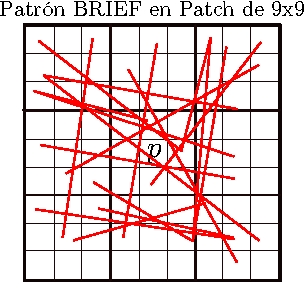
\includegraphics[width=\columnwidth]{./images/camera/brief}
		\end{figure}
	\end{minipage}\hfill{}
	\begin{minipage}[t]{0.6\columnwidth}
		\centering
		256 Comparaciones entre píxeles (1 a 1)
		\begin{equation*}
			\tau(p;x,y) =
			\begin{cases}
				1 & \text{if $p(x) < p(y)$}\\
				0 & \text{otherwise}\\
			\end{cases}     
		\end{equation*}
		$s = \overbrace{01010010101110010...}^{256\ \text{bits}}$
	\end{minipage}
	\begin{block}{Matching distance}
		$\text{Hamming distance} = sum (XOR(s_{1}, s_{2}))$
	\end{block}
	\note{utilizamos la distancia de hamming para la distancia de matcheo entre descriptores.}
\end{frame}

\begin{frame}
	\frametitle{Matcheo de keypoints}
	\footnotesize
	
\end{frame}

\begin{frame}
	\frametitle{RANSAC: Random Sample Consensus}
	\footnotesize
	
	\begin{itemize}
		\item Permite encontrar un modelo que ajusta datos en presencia de ruido y outliers
		\item Separa el conjunto de datos entre inliers y outliers
%		\item Encuentra la mejor partición de puntos en un conjunto de inliers y outliers. Estima un modelo utilizando el conjunto de inliers.
		\item Ejemplo: dado un conjunto de puntos 2D, ajustar una línea 
	\end{itemize}
	
	\begin{figure}
		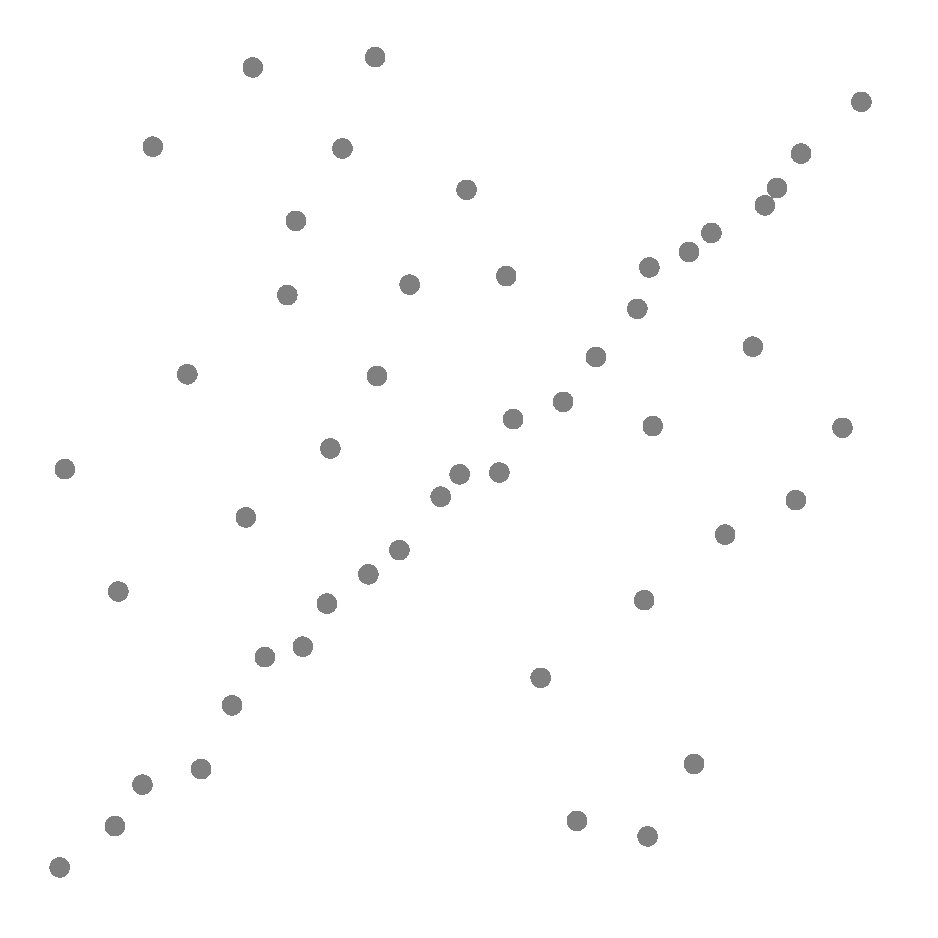
\includegraphics[width=0.5\textwidth]{./images/ransac_points.pdf}
	\end{figure}

	\TODO{hacer imágenes similares a las del vídeo: https://youtu.be/ebMyBbkkHWk}
	
\end{frame}


\begin{frame}
	\frametitle{RANSAC: Random Sample Consensus}
	\footnotesize
	
	\TODO{hacer imágenes similares a las del vídeo: https://youtu.be/ebMyBbkkHWk}
	
	\begin{figure}
		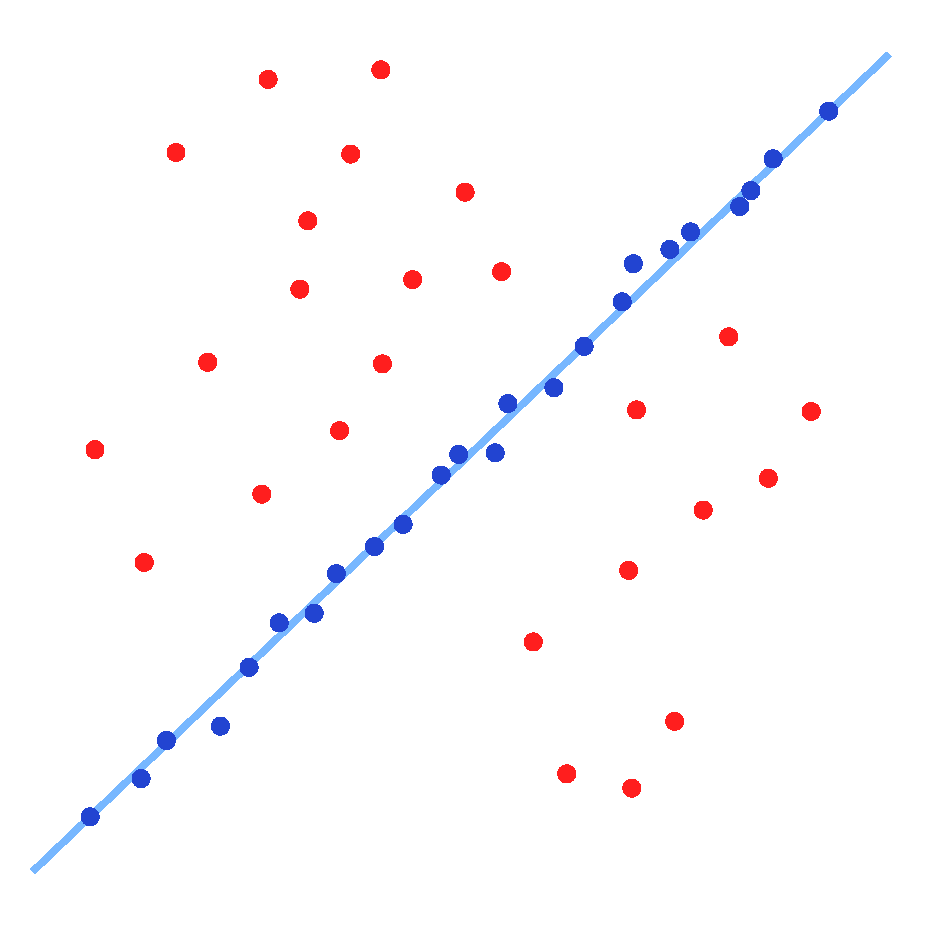
\includegraphics[width=0.5\textwidth]{./images/ransac_fitted_line.pdf}
	\end{figure}
	
\end{frame}
\begin{frame}
	\frametitle{RANSAC: Random Sample Consensus}
	\footnotesize

	\begin{enumerate}
		\item {\bf Samplear} de manera aleatoria el número de puntos requerido para ajustar el modelo.
		\item {\bf Computar} el modelo usando los datos sampleados
		\item {\bf Contar} el número de inliers y quedarse con el modelo que mejor ajusta los datos
		\item Iterar puntos 1-3 hasta que el mejor modelo es hallado
	\end{enumerate}

\end{frame}

\begin{frame}
	\frametitle{RANSAC: Random Sample Consensus}
	\footnotesize
	
	Pero...¿cuantas iteraciones realizar?
	
	\begin{itemize}
		\item Número de puntos sampleados $s$ (número de puntos mínimos requeridos para ajustar el modelo)
		\item Ratio de outliers $e = \dfrac{\# outliers}{\# puntos totales}$
		\item Número de intentos $T$.
		Elegimos $T$, con probabilidad $p$ de éxito (la probabilidad de al menos obtener un muestreo aleatorio libre de outliers en las $T$ iteraciones).
	\end{itemize}
	
	Probabilidad de fallar en una iteración, es decir de no seleccionar todos inliers.
	\begin{equation*}
		1-p = 1 - (1 - e)^{s}
	\end{equation*} 
	\note{(1-e)^s es la probabilidad de seleccionar todos inliers}
	
	
	Probabilidad de fallar en $T$ iteraciones, es decir seleccionar un outlier en todas las iteraciones.
	
	\begin{equation*}
		1-p = (1 - (1 - e)^{s})^{T}
	\end{equation*} 
	despejando $T$,
	\begin{equation*}
		T = \dfrac{\log(1-p)}{\log(1-(1-e)^{s})}
	\end{equation*} 
	
\end{frame}

\begin{frame}
	\frametitle{RANSAC: ventajas y desventajas}
	\footnotesize
	Ventajas:
	\begin{itemize}
		\item Robusto en presencia de outliers
		\item funciona bien para modelos de 1 a 10 parámetros (dependiendo del número de outliers)
		\item Fácil de implementar y entender
	\end{itemize}
	Ventajas:
	\begin{itemize}
		\item El tiempo computacional crece rápido con el porcentaje de outliers y el número de parámetros necesarios para ajustar el modelo
		\item No es bueno para obtener múltiples modelos (e.g. ajustar más de una línea en 2D)
	\end{itemize}
\end{frame}

\begin{frame}
	\frametitle{Cámara - Modelo Pin-Hole}
	
	\note{Ver libro de Sigwart. Seccion 4.2.3.2}
	\note{material sacado de mi tesis}
	
	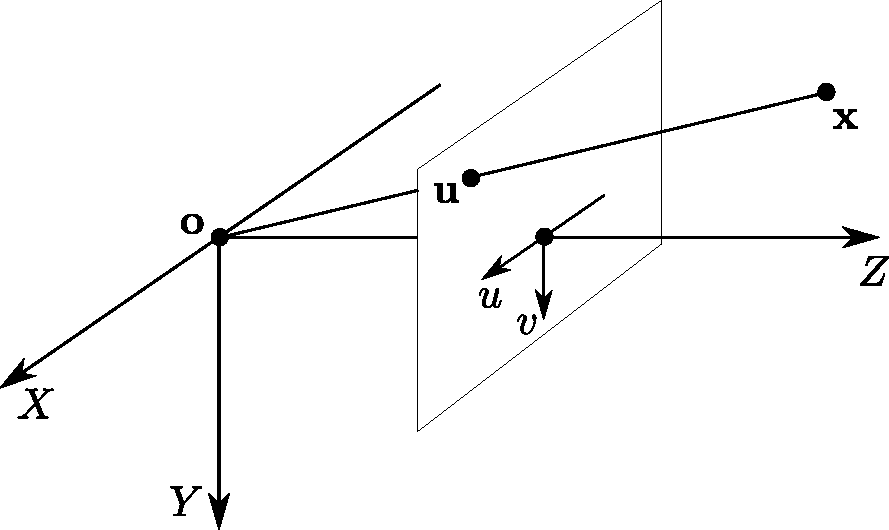
\includegraphics[width=0.4\columnwidth]{images/camera/pinhole_camera_model.pdf}
	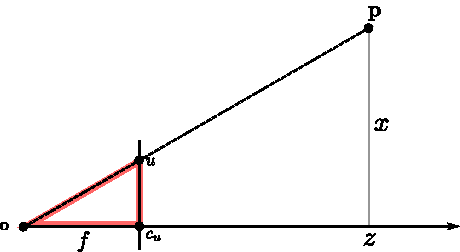
\includegraphics[width=0.4\columnwidth]{images/camera/pinhole_camera_model2.pdf}
	\footnotesize
	
	\begin{block}{Principio de funcionamiento}
		En el modelo de cámara pinhole, el punto de la imagen $\imagePoint=\begin{bmatrix}u & v\end{bmatrix}^{\top}$ se determina como la intersección entre el plano de la imagen y el rayo que une el punto del mundo $\point =\begin{bmatrix}x & y & z\end{bmatrix}^{\top}$ y el centro de proyección $\cameraCenter$.
	\end{block}
	
	Denotamos con $\homo{\point}=\begin{bmatrix}x & y & z & 1\end{bmatrix}^{\top}$ la representación homogénea de un punto $\point=\begin{bmatrix}x & y & z\end{bmatrix}^{\top}$. Ahora, definimos el modelo de cámara:
	\begin{equation*}
		\imagePoint=f\proj(\cameraPoint)+\principalPoint
	\end{equation*}
	
	donde $f$ es la distancia focal, $\principalPoint$ es el punto principal, $\cameraPoint$ es el punto en el sistema de coordenadas de la cámara y la función $\proj:\mathbb{R}^{n}\rightarrow\mathbb{R}^{n- 1}$ se puede usar para transformar puntos de coordenadas homogéneas a no homogéneas, y también se puede usar para proyectar puntos del espacio 3D al plano de imagen 2D.	
\end{frame}

\begin{frame}
	\frametitle{Cámara - Modelo Pin-Hole}
	
	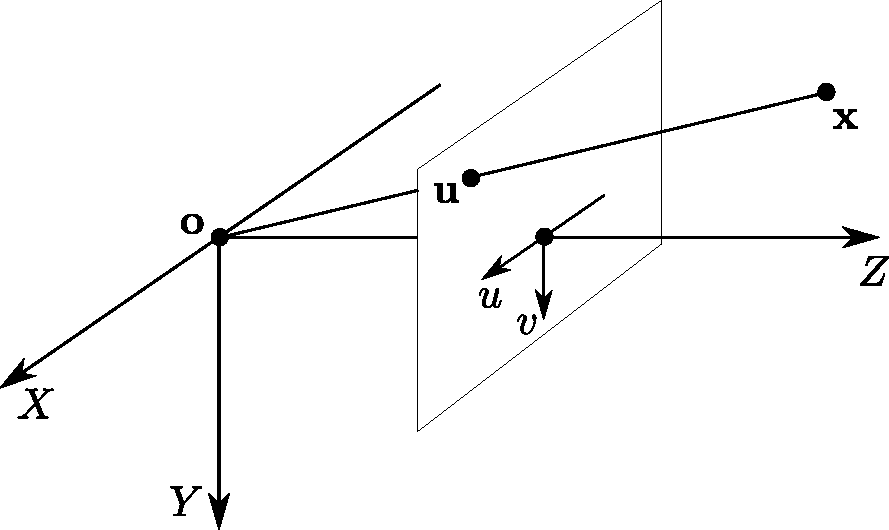
\includegraphics[width=0.4\columnwidth]{images/camera/pinhole_camera_model.pdf}
	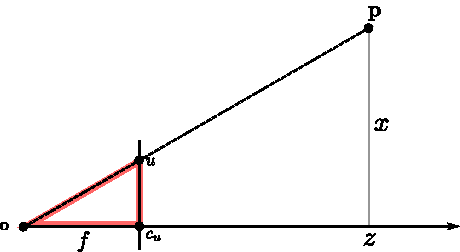
\includegraphics[width=0.4\columnwidth]{images/camera/pinhole_camera_model2.pdf}
	\footnotesize
	
	\begin{equation*}
		\proj(\vec{a})=
		\frac{1}{a_{n}}\begin{bmatrix}a_{1}\\
			\vdots\\
			a_{n-1}
		\end{bmatrix}.
	\end{equation*}
	
	Por ejemplo, si $\point=\begin{bmatrix}x & y & z\end{bmatrix}^{\top}$, entonces $\proj(\point)=\begin{bmatrix}x/z & y/z\end{bmatrix}$.
	
	Se puede ver que $x/z=u/f$. Análogamente podemos decir que $y/z=v/f$. De estas ecuaciones podemos ver que $u=f(x/z)$ y que $v=f(y/z)$, por lo que la ecuación [eq:proyección] se cumple.
	
\end{frame}


\begin{frame}
	\frametitle{Cámara - Modelo Pin-Hole}
	
	\footnotesize
	
	En el caso general, la cámara no está ubicada en el centro del sistema de coordenadas del mundo. Tenemos que agregar esta transformación entre el mundo y los sistemas de coordenadas de la cámara a la ecuación anterior, lo que da como resultado
	
	\begin{equation*}
		\imagePoint=f\proj(\proj(\seMatrix^{\mathrm{c}\mathrm{w}}\homoWorldPoint))+\principalPoint,
	\end{equation*}
	
	donde $\seMatrix^{\mathrm{c}\mathrm{w}}$ es una matriz de transformación que transforma elementos geométricos del marco de coordenadas del mundo $\mathrm{W}$ al marco de coordenadas de la cámara $\mathrm{C}$. Esto es,
	\begin{equation*}
		\homoCameraPoint=\seMatrix^{\mathrm{c}\mathrm{w}}\homoWorldPoint.
	\end{equation*}
	
\end{frame}

\begin{frame}
	\frametitle{Cámara - Modelo Pin-Hole}
	
	\footnotesize
	
	En particular, $\seMatrix^{\mathrm{c}\mathrm{w}}$ es una transformación que pertenece al Lie Group SE(3), el grupo de movimientos de cuerpo rígido en el espacio 3D. Por lo tanto, $\seMatrix^{\mathrm{c}\mathrm{w}}$ se define como
	$\seMatrix^{\mathrm{c}\mathrm{w}}=
	\begin{bmatrix}\rotation & \translation\\
		\vec{0} & 1
	\end{bmatrix}$ donde $\rotation$ es una matriz de rotación y $\translation$ es un vector de traslación. Observe que una de las ventajas de trabajar con coordenadas homogéneas es que permite utilizar el álgebra de Grupos de Lie SE(3).
	
	Existe una notación de matriz para el modelo de cámara pin-hole que también se usa comúnmente en visión por computadora.
	\begin{equation*}
		\projectionMatrix=\intrinsicMatrix\begin{bmatrix}\rotation & \translation\end{bmatrix}
	\end{equation*}
	
	donde $\projectionMatrix$ es la matriz de proyección y $\intrinsicMatrix$ es la matriz de calibración. La matriz de calibración se define como,
	
	\begin{equation*}
		\intrinsicMatrix=
		\begin{bmatrix}f & 0 & c_{u}\\
			0 & f & c_{v}\\
			0 & 0 & 1
		\end{bmatrix},
	\end{equation*}
	
\end{frame}

\begin{frame}
	\frametitle{Cámara - Modelo Pin-Hole}
	
	\footnotesize
	
	Siendo $\begin{bmatrix}c_{u} & c_{v}\end{bmatrix}^{\top}$ la posición del punto principal. Entonces, usando la matriz de proyección $\projectionMatrix$, el punto del mundo $\worldPoint$ se asigna al punto imagen $\imagePoint$ por
	\begin{equation*}
		\imagePoint=\proj{(\projectionMatrix\homoWorldPoint)}.
	\end{equation*}
	
\end{frame}


\begin{frame}
	\frametitle{Distorción}
	
	\footnotesize
	
	Previamente, consideramos que el modelo de cámara pin-hole es perfectamente lineal, es decir, el punto en el mundo, el punto en la imagen y el centro óptico son colineales.
	
	Esta suposición no es cierta en la práctica porque hay una distorsión radial en la imagen producida por la lente de la cámara real.
	
	\begin{figure}[!h]
		\centering
		\subfloat[Sin distorción]
		{
			
\includegraphics[width=0.2\columnwidth]{images/camera/no_distortion.pdf}
		}
		\subfloat[Barrel distortion]
		{
			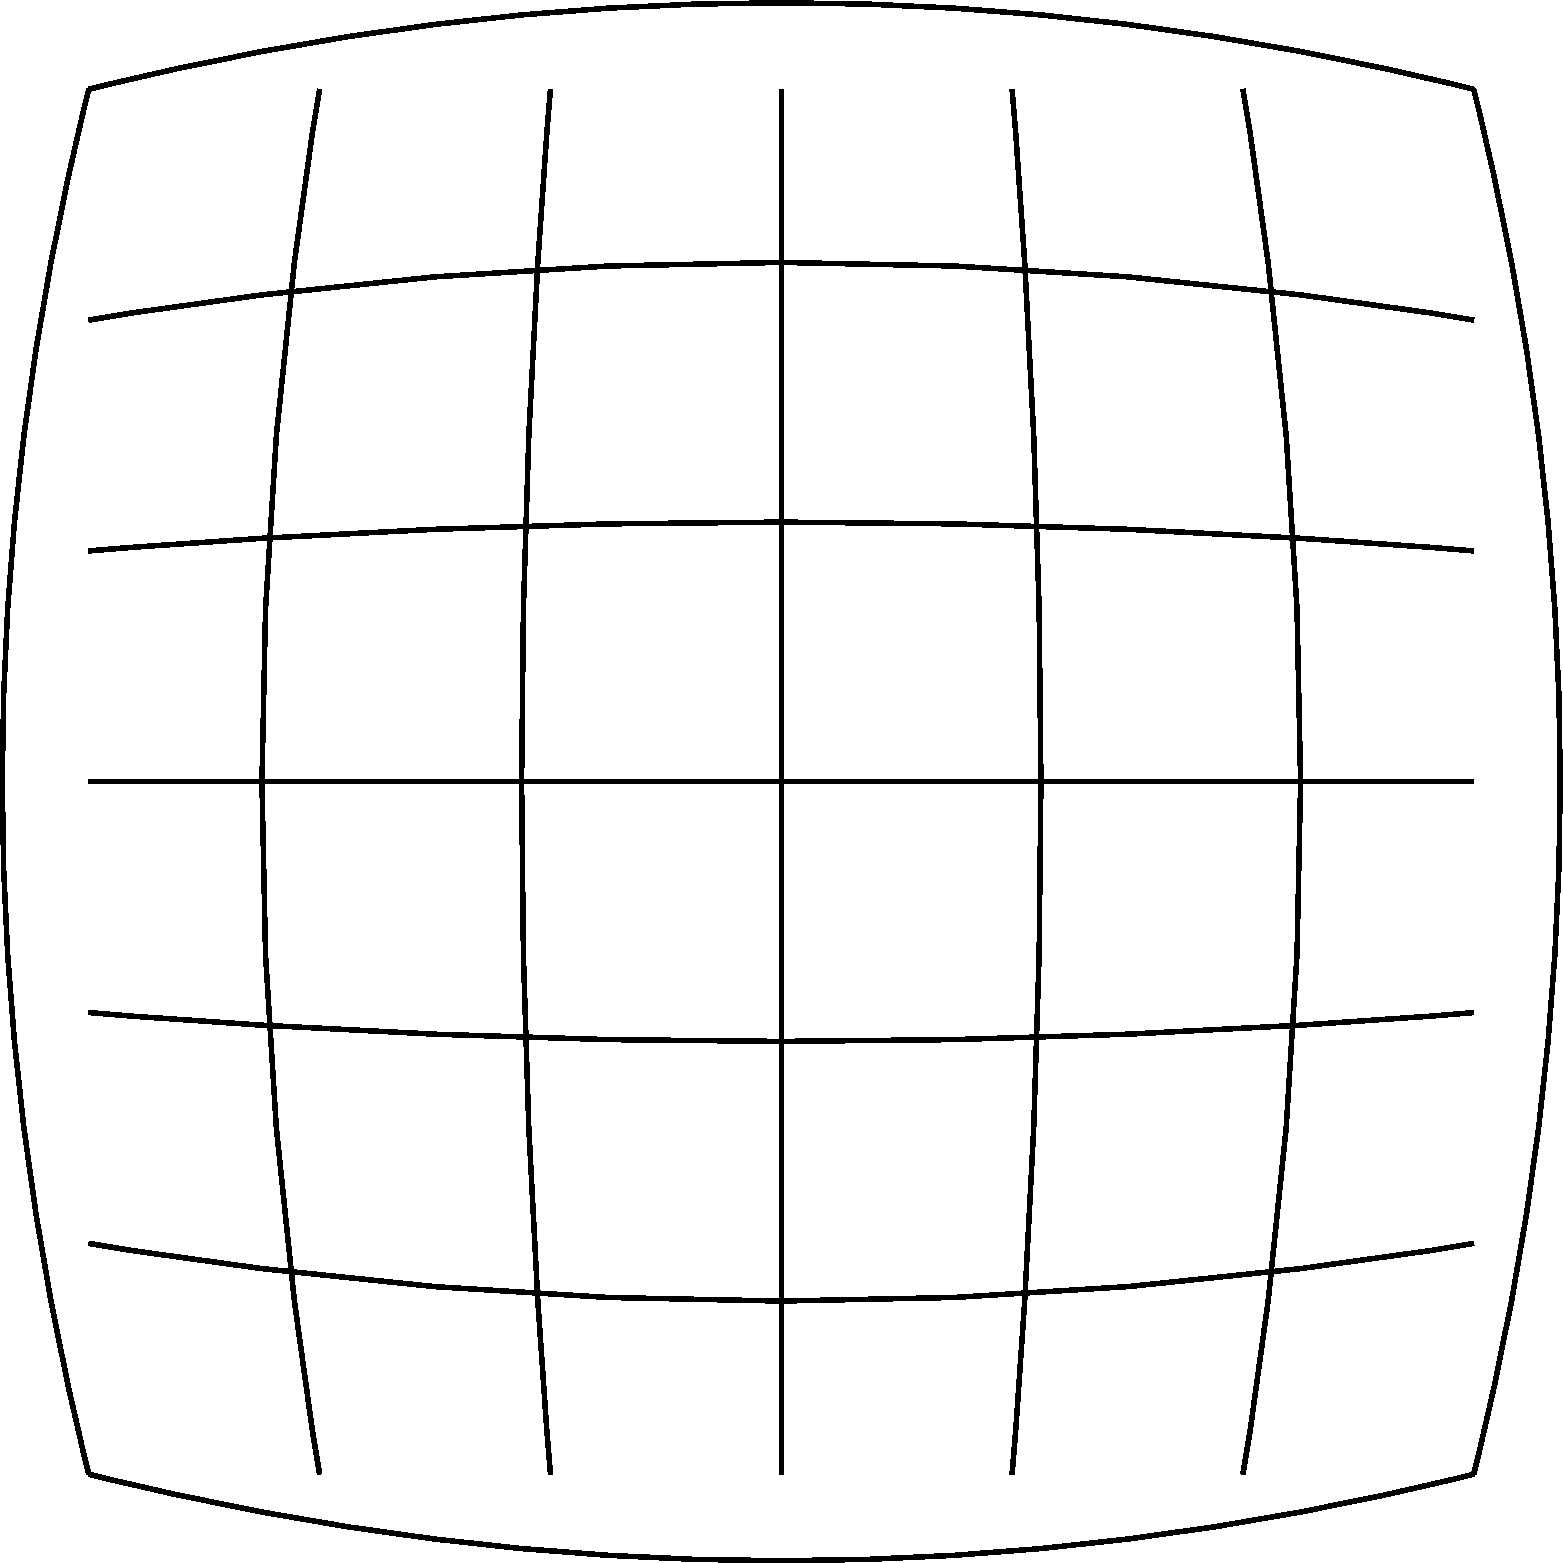
\includegraphics[width=0.2\columnwidth]{images/camera/barrel_distortion.pdf}
		}
		\subfloat[Pincushion distortion]
		{
			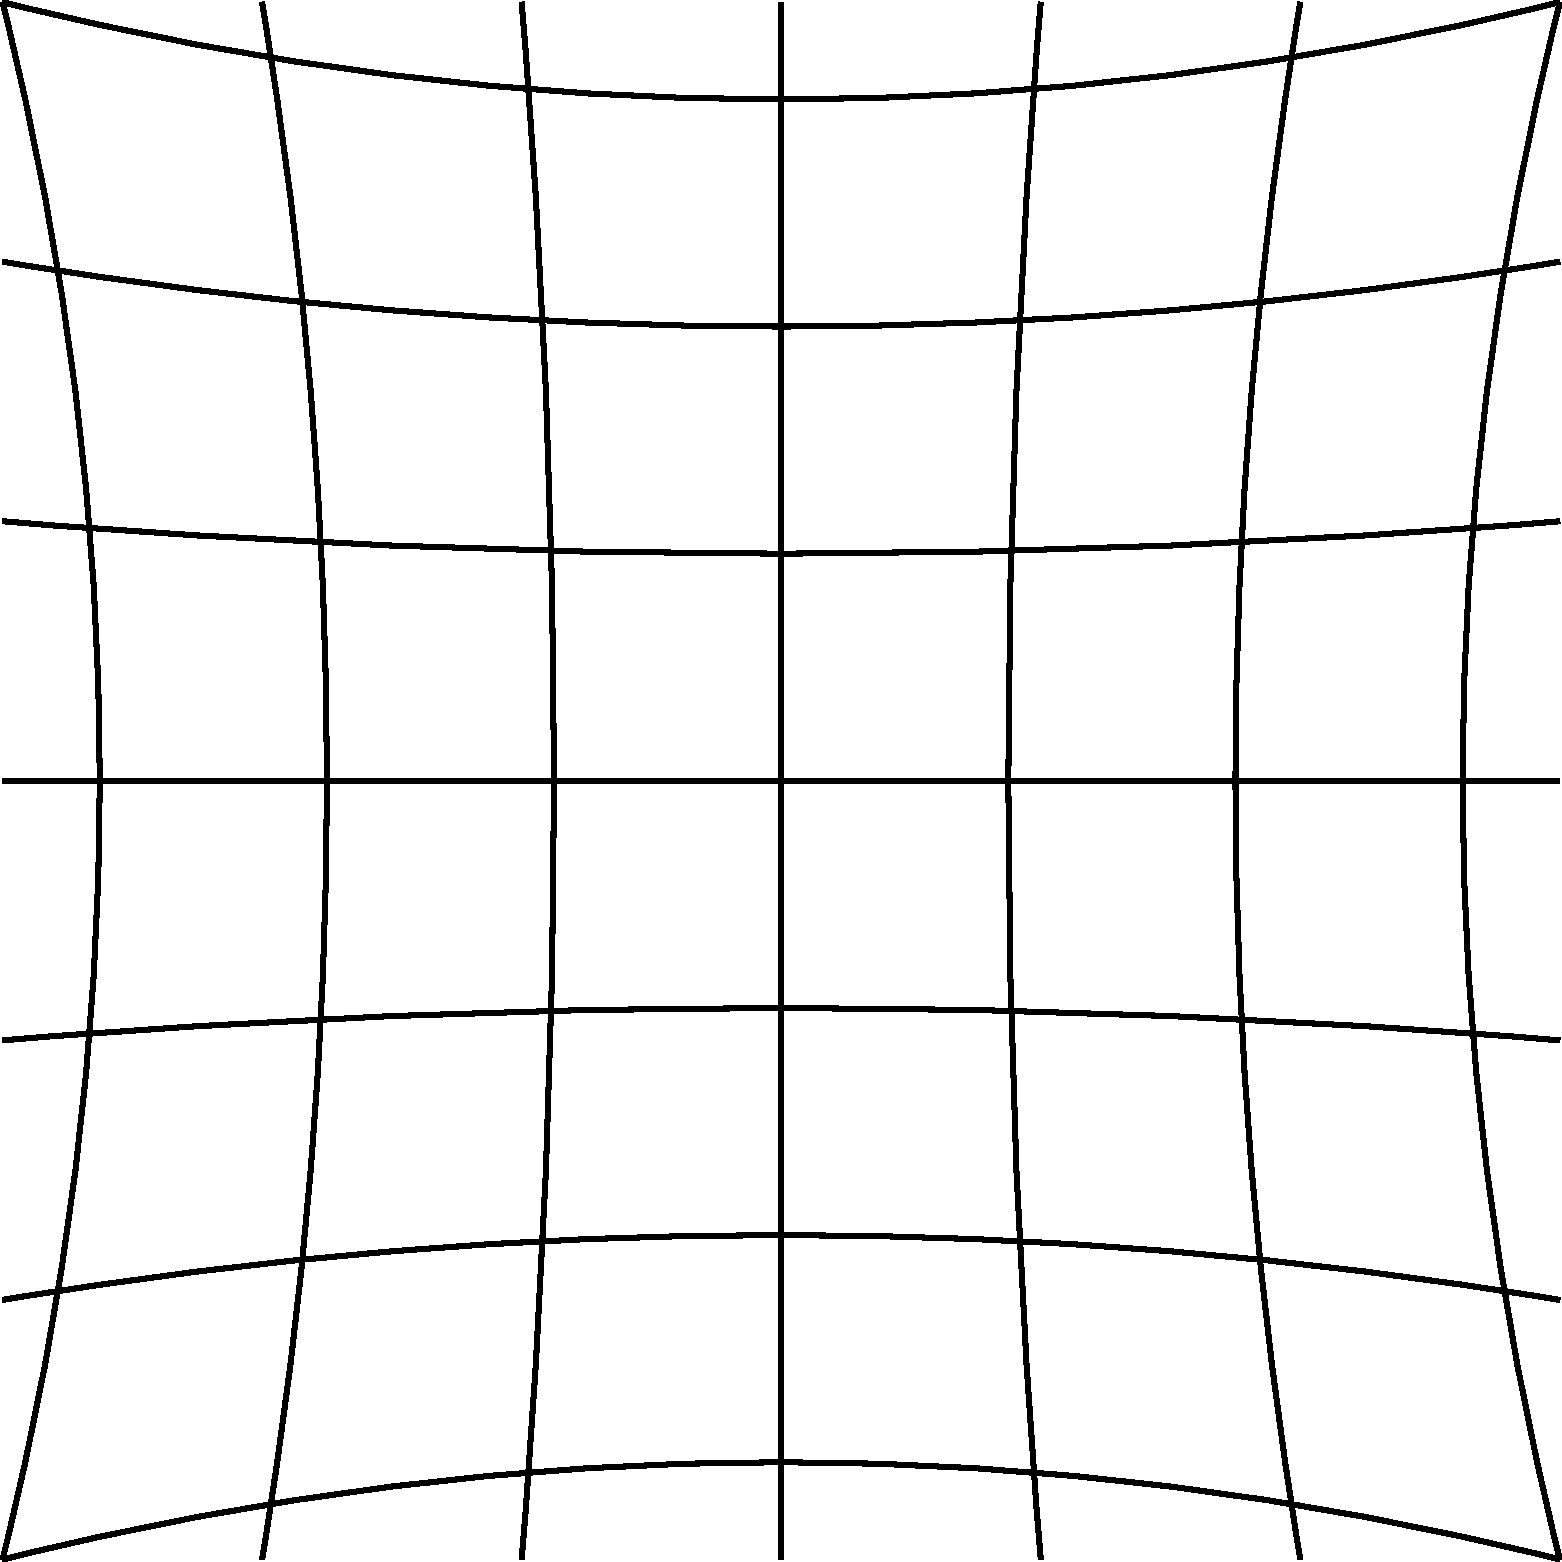
\includegraphics[width=0.2\columnwidth]{images/camera/pincushion_distortion.pdf}
		}
		\subfloat[Mustache distortion]
		{
			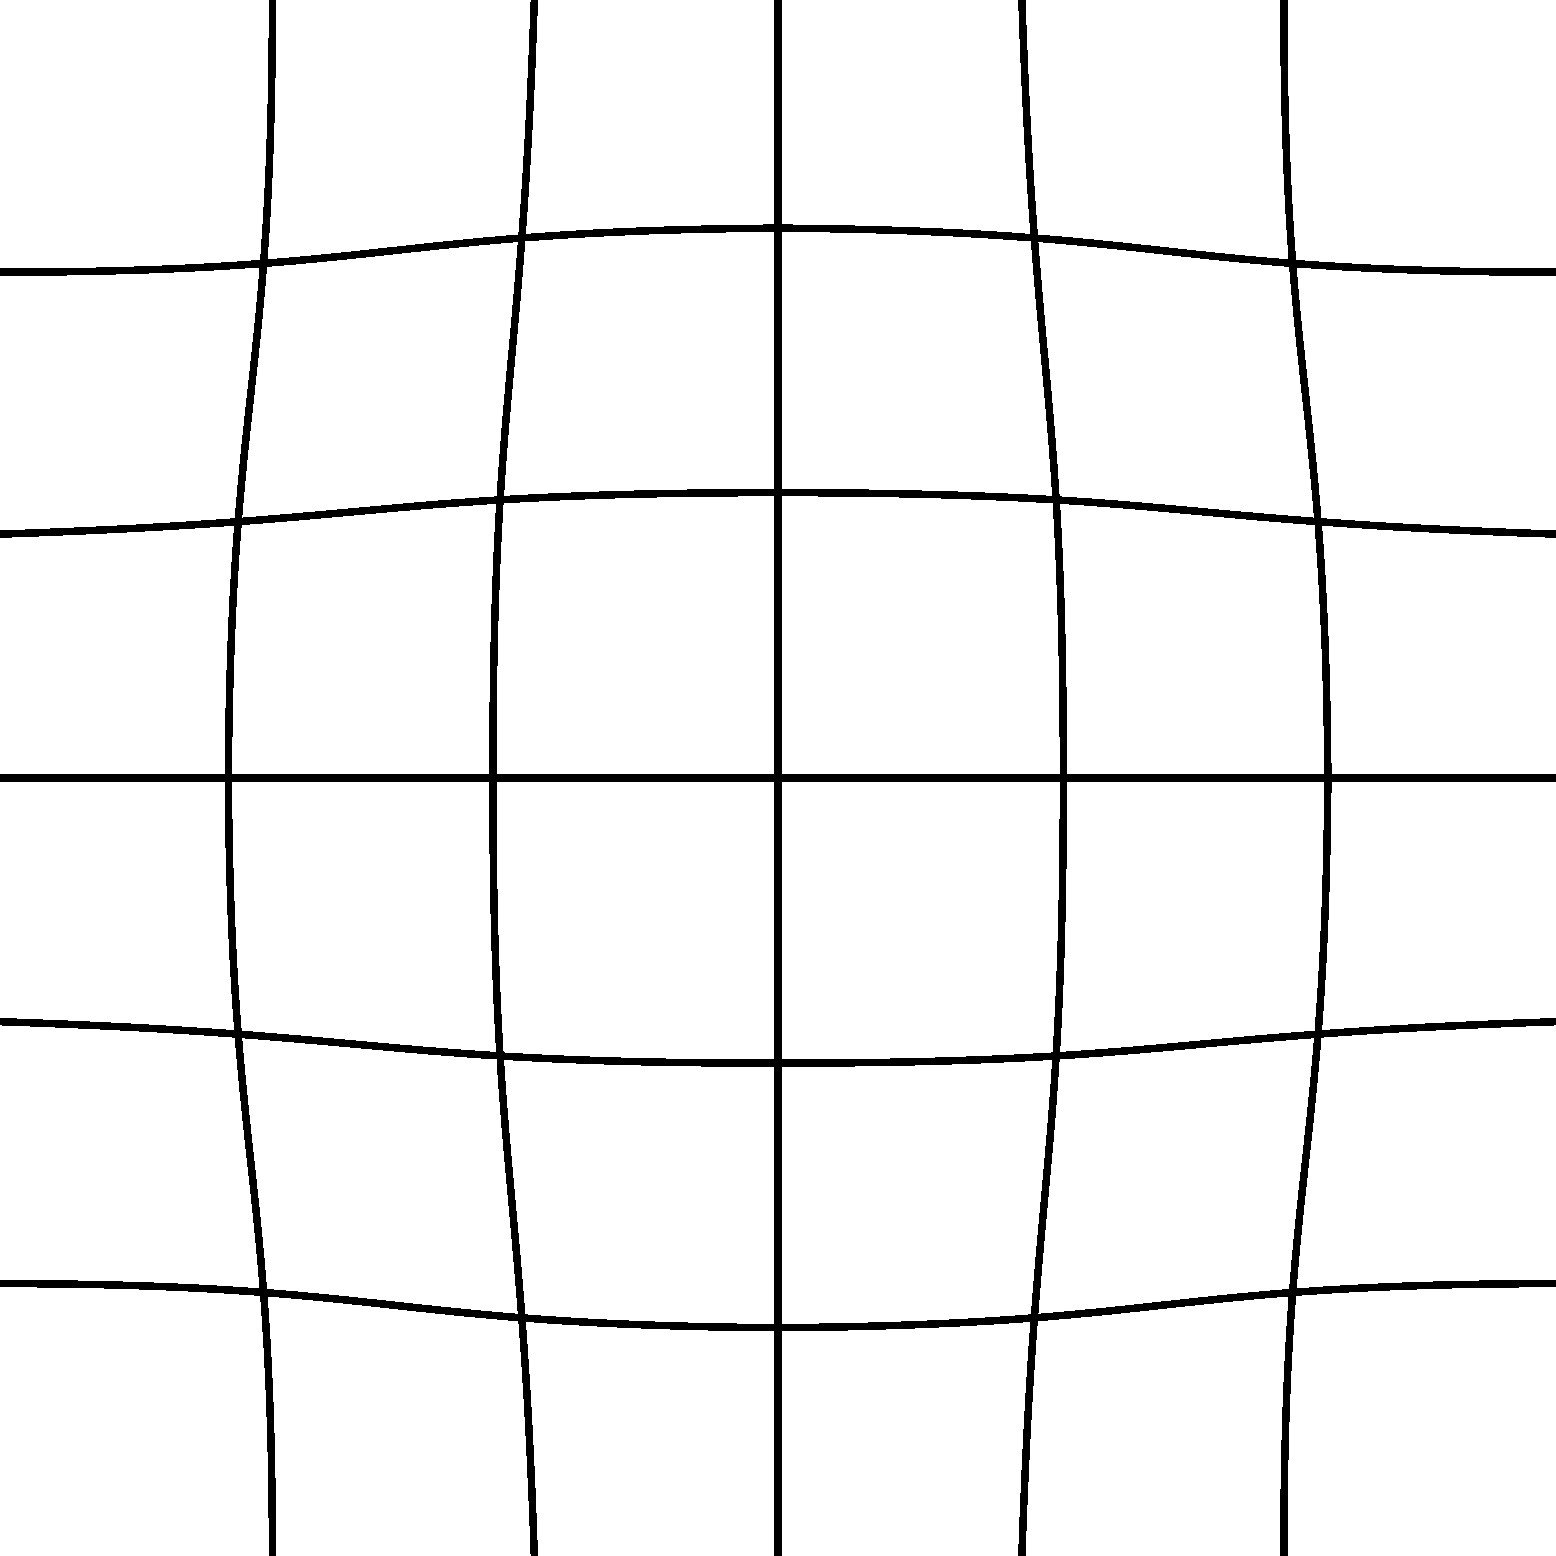
\includegraphics[width=0.2\columnwidth]{images/camera/mustache_distortion.pdf}
		}
	\end{figure}
	
\end{frame}


\begin{frame}
	\frametitle{Distorción}
	
	Para corregir esta distorsión se calcula un modelo de distorsión radial que relaciona los puntos de la imagen de la imagen real con los puntos ideales, los que se habrían obtenido bajo una cámara lineal perfecta. De esta forma, la cámara se puede representar con un modelo pin-hole lineal. En la figura es posible observar la imagen cruda (distorsionada) tomada por la cámara y la imagen después de la desdistorsión.
	
	\begin{figure}[!h]
		\centering
		\subfloat[Imagen distorcionada]
		{
			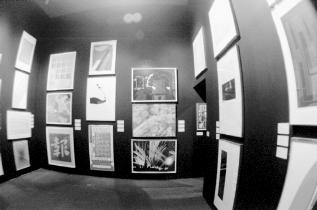
\includegraphics[width=0.45\columnwidth]{images/camera/distorted_image.png}
		}
		\subfloat[Imagen desdistorcionada]
		{
			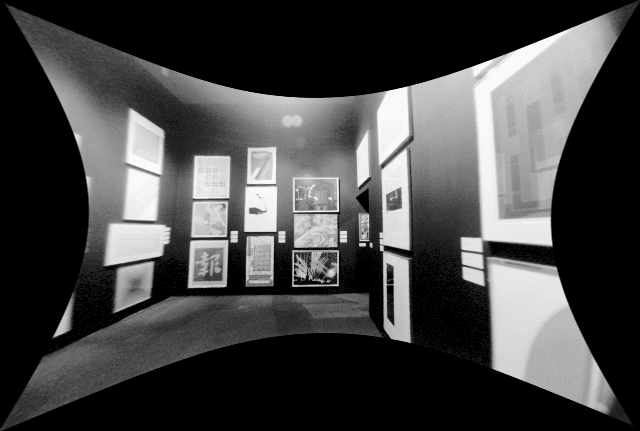
\includegraphics[width=0.45\columnwidth]{images/camera/undistorted_image.png}
		}
	\end{figure}
	
\end{frame}


\begin{frame}
	\frametitle{Distorción}
	
	\footnotesize
	
	Dado el punto proyectado real y el punto ideal, el efecto de distorsión radial se puede modelar mediante
	\begin{equation}
		\begin{bmatrix}u_{d}\\
			v_{d}
		\end{bmatrix}=L(\tilde{r})\begin{bmatrix}\tilde{u}\\
			\tilde{v}
		\end{bmatrix}
	\end{equation}
	
	donde, 
	$\begin{bmatrix}\tilde{u}\\ 
		\tilde{v}
	\end{bmatrix}$
	es la posición ideal de la imagen referida al centro de la imagen (que obedece a la proyección lineal);
	$\begin{bmatrix}u_{d}\\
		v_{d}
	\end{bmatrix} $
	es la posición real de la imagen después de la distorsión radial; $\tilde{r}$ es la distancia radial $\sqrt{\tilde{u}^{2}+\tilde{v}^{2}}$ desde el centro para la distorsión radial, y $L(\tilde{r})$ es una factor de distorsión, que es una función del radio $\tilde{r}$.
\end{frame}

\begin{frame}
	\frametitle{Distorción}
	
	\footnotesize
	
	Finalmente, la corrección se puede representar en coordenadas de píxeles como
	\begin{equation*}
		\begin{aligned}\hat{u} & =u_{c}+L(r)(u-u_{c})\\
			\hat{v} & =v_{c}+L(r)(v-v_{c})
		\end{aligned}
	\end{equation*}
	
	donde 
	$\begin{bmatrix}u\\
		v
	\end{bmatrix}$ 
	son las coordenadas medidas, 
	$\begin{bmatrix}\tilde{u}\\
		\tilde{v}
	\end{bmatrix}$ 
	son las coordenadas corregidas, y 
	$\begin{bmatrix}u_{c}\\
		v_{c}
	\end{bmatrix}$ 
	es el centro de distorsión radial, con $r^{2}=(u-u_{c})^{2}+(v-v_{c})^{2}$.
	
	El factor de distorsión $L(r)$ esta definido solo por valores positivos de $r$ y $L(0)=1$. En la práctica, $L(r)$ es aproximado por la expansión de Taylor
	
	\begin{equation*}
		L(r)=1+k_{1}r+k_{2}r^{2}+k_{3}r^{3}+\ldots.
	\end{equation*}
	
	Los coeficientes $\left\{ k_{1},k_{1},k_{1},\ldots,u_{c},v_{c}\right\}$ se consideran parte de la calibración interna de la cámara. Con frecuencia, el punto principal se utiliza como centro de la distorsión radial, aunque no es necesario que coincidan exactamente. Los coeficientes de corrección, junto con la matriz de calibración de la cámara, especifican el mapeo desde un punto de la imagen hasta un rayo en el sistema de coordenadas de la cámara y se denominan parámetros intrínsecos.
\end{frame}



\begin{frame}
	\frametitle{Geometría Epipolar}
	\footnotesize
	
	\begin{itemize}
		\item La restricción epipolar puede ser computada por medio de puntos 2D en la imagen cuando la pose relative de la cámara es conocida ($\transform{r}{l}$, por ejemplo una cámara estéreo)
		\item El plano epipolar es definido por $\imagePoint_{l}$ y los dos dentros óptico de las cámaras $\cameraCenter_{l}$ y $\cameraCenter_{r}$
		\item La línea epipolar es la intersección del plano epipolar y el plano de la imagen derecha.
		\item La restricción epipolar codifica que $\imagePoint_{r}$ debe estar ubicado sobre la linea epipolar en la imagen derecha.
	\end{itemize}

	\begin{equation*}
		\homoImagePoint_{l}^{\top} \essentialMatrix \homoImagePoint_{r}^{\top} = 0,
	\end{equation*}
	donde $\essentialMatrix = \transform{l}{r}$, y se denomina \emph{Essential Matrix}
	
	La línea epipolar permite que restrinjamos la búsqueda de correspondencias visuales entre dos cámaras.
	
	\TODO{renombrar variables en imágenes}
	
	\begin{figure}
		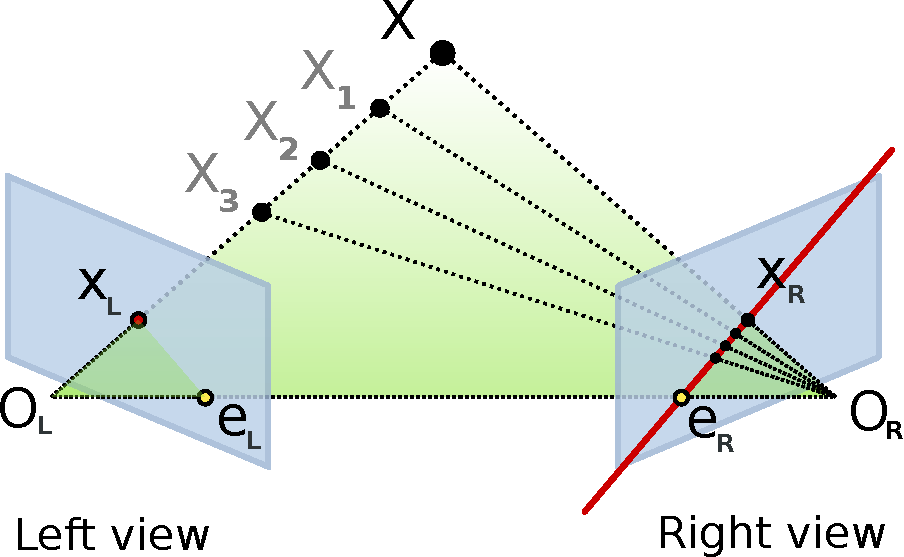
\includegraphics[width=0.4\textwidth]{./images/epipolar_geometry.pdf}
	\end{figure}
	
\end{frame}

\begin{frame}
	\frametitle{Estimación de movimiento}
	\footnotesize
	\TODO{Hacer imágenes para cada caso}
	
	2D-2D
    \begin{columns}
	\begin{column}{0.7\textwidth}
		\begin{itemize}
		\item Error de reproyección:
		\[
		f(\transform{a}{b}, \mapPointsSet)= \sum_{i=1}^{N} \Vert \measurement_{a,i} - \prediction^{\mathrm{s}}(\transform{a}{\worldCoordSystem},\worldPoint_{i}) \Vert^{2} + \Vert \measurement_{b,i} - \prediction^{\mathrm{s}}(\inverse{\transform{a}{b}}\transform{a}{\worldCoordSystem},\worldPoint_{i}) \Vert^{2}
		\]
		\item Algoritmos lineales: 8-point, 5-point
		\end{itemize}
	\end{column}
	\begin{column}{0.3\textwidth}
	    \begin{figure}
			\def\svgwidth{\columnwidth}
			\import{./images/}{tracking_reprojection_error_after.pdf_tex}
		\end{figure}
	\end{column}
	\end{columns}

	3D-2D
    \begin{columns}
	\begin{column}{0.7\textwidth}
		\begin{itemize}
			\item Error de reproyección:
			\[
			f(\transform{\worldCoordSystem}{a}, \mapPointsSet)= \sum_{i=1}^{N} \Vert \measurement_{a,i} - \prediction(\inverse{\transform{\worldCoordSystem}{a}},\worldPoint_{i}) \Vert^{2}
			\]
			\item Algoritmos lineales: DLT, PnP
		\end{itemize}
	\end{column}
	\begin{column}{0.3\textwidth}
		\begin{figure}
			\def\svgwidth{\columnwidth}
			\import{./images/}{tracking_reprojection_error_after.pdf_tex}
		\end{figure}
	\end{column}
	\end{columns}
	3D-3D
	\begin{columns}
		\begin{column}{0.7\textwidth}
			\begin{itemize}
				\item Error de reproyección:
				\[
				f(\transform{a}{b})= \sum_{i=1}^{N} \Vert \pointCoord{a}_{i} - \transform{a}{b} \pointCoord{b}_{i} \Vert^{2}
				\]
				\item Algoritmos lineales: Atun, Horn
			\end{itemize}
		\end{column}
		\begin{column}{0.3\textwidth}
			\begin{figure}
				\def\svgwidth{\columnwidth}
				\import{./images/}{tracking_reprojection_error_after.pdf_tex}
			\end{figure}
		\end{column}
	\end{columns}

\end{frame}

\begin{frame}
	\frametitle{Estimación de movimiento 2D-2D}
	\footnotesize
	
	\begin{itemize}
		\item dados los matches 2D-2D $\{(\measurement_{a}, \measurement_{b})_{i}\}$ de puntos 3D desconocidos $\mapPointsSet_{i}$ encontrar el movimiento relativo $\transform{a}{b}$ entre los frames.
		\item Error de reproyección (Bundle Adjustment):
		\[
		f(\transform{a}{b}, \mapPointsSet)= \sum_{i=1}^{N} \Vert \measurement_{a,i} - \prediction^{\mathrm{s}}(\transform{a}{\worldCoordSystem},\worldPoint_{i}) \Vert^{2} + \Vert \measurement_{b,i} - \prediction^{\mathrm{s}}(\inverse{\transform{a}{b}}\transform{a}{\worldCoordSystem},\worldPoint_{i}) \Vert^{2}
		\]
		Se puede optimizar con métodos no lineales pero requieren de una buena semilla inicial. Es no convexo, solución no única (ambigüedadad de escala)
		\item Se puede utilizar un enfoque algebraico basado en geometría epipolar para obtener la transformación relativa (a un factor de escala) sin explicitamente computar la posición de los puntos 3D: algoritmos 8-point y 5-point.
		\item Aplicaciones:
		\begin{itemize}
			\item Filtrar matches con RANSAC
			\item Inicializar una sistemas de SLAM monocular / SfM
		\end{itemize}
	\end{itemize}
\end{frame}

\begin{frame}
	\frametitle{Estimación de movimiento 3D-2D}
	\footnotesize
	
	\begin{itemize}
		\item Dado un conjunto de correspondencias 3D-2D $\{(\worldPoint, \measurement_{a})_{i}\}$ queremos encontrar la pose $\transform{w}{a}$ de la cámara en el mundo.
		\item Error de reproyección:
		\[
		f(\transform{\worldCoordSystem}{a}, \mapPointsSet)= \sum_{i=1}^{N} \Vert \measurement_{a,i} - \prediction(\inverse{\transform{\worldCoordSystem}{a}},\worldPoint_{i}) \Vert^{2}
		\]
		Se puede optimizar con métodos no lineales pero requieren de una buena semilla inicial. Es no convexo, solución no única (ambigüedad de escala)
		\item Este problema es conocido como \emph{Perspective-n-Points} (PnP) y existen diferentes enfoques para resolverlo:
		\begin{itemize}
			\item Direct Linear Transform (DLT)
			\item EPnP
			\item OPnP
		\end{itemize}
		\item Aplicaciones:
		\begin{itemize}
			\item Localización de una cámara dado un mapa de puntos (tracking)
		\end{itemize}
	\end{itemize}
	
\end{frame}

\begin{frame}
	\frametitle{Estimación de movimiento 3D-3D}
	\footnotesize
	
	\begin{itemize}
		\item Dado un conjunto de correspondencias 3D en dos sistemas de coordenadas distintos: $\{(\pointCoord{a}, \pointCoord{b})_{i}\}$ queremos encontrar la transformación relativa $\transform{a}{b}$.
		\item Error geométrico 3D:
		\[
		f(\transform{a}{b})= \sum_{i=1}^{N} \Vert \pointCoord{a}_{i} - \transform{a}{b} \pointCoord{b}_{i} \Vert^{2}
		\]
		Corresponde a alineamiento de nube de puntos por mínimos cuadrados.
		\item Solución cerrada, eg.g Arun et al, 1987
		\item Aplicaciones:
		\begin{itemize}
			\item Obtención de movimiento relativo para cámaras estéreo (mediante el uso de puntos triangulados) o RGB-D (mediciones con profundidad)
			\item Corrección de Loop Closure (variante con estimación de escala para SLAM monocular)
		\end{itemize}
	\end{itemize}
	
\end{frame}

\begin{frame}
	\frametitle{Tipos de transformaciones}
	\footnotesize
	
\end{frame}

\begin{frame}
	\frametitle{Calibración de cámara}
	\footnotesize
	
	
\end{frame}



